\chapter{Avoiding Undesirable Consequences}
\textit{\textbf{Imagine a human user learning to use a new software application. In the beginning, the user is more likely to make mistakes because he may not have all the information to work with the software. In another instance, while performing routine tasks on the computer, the user may receive a phishing email appearing to be from a well-known and trusted source, requesting personal information.}}
The two scenarios highlight how the routine tasks performed by human users can sometimes have unintended, perhaps dangerous consequences.
The same can occur when a software agent executes a task in a complex environment, where the agent may be subverted by hidden information or by a nefarious agent acting as an adversary. 
In the case of a human user, the cognitive load imposed by the task may be an additional impediment for the user to find a sequence of actions that completes the task safely.
User error or actions of nefarious agents may cause plans to accomplish the intended goal become vulnerable to undesirable consequences. 
Therefore, when working in an unfamiliar environment, it is important to have a system in place to recognize in advance when the software agent or the human user is executing a plan that will result in an undesirable consequence, and upon recognition, guide the agent (or the human user) toward the goal while avoiding the undesirable consequence. 
We propose intervention as a utility for online assistive agents and safety critical decision making for human users.
As illustrated in Figure~\ref{fig:stages}, we model intervention as a two stage process. 
The environment is modeled as a state transition system. 
The agent (or the human user), in order to achieve a desirable outcome, executes actions ($a_1$, $a_2, \ldots$) that change environment from one state to the next ($S_0, S_1, S_2, \ldots$). 
For simplicity, henceforth we refer to the agent in the environment as \textit{the user}.
Some states in the environment are undesirable and the user does not have the ability to recognize them. 
The intervening agent, henceforth referred to as \textit{the observer}, wants to help the user in the environment avoid the undesirable state.

In the first stage of the intervention process, which we refer to as \textit{\textbf{the undesirable state recognition process}}, the observer monitors what the user doing.
The observations may consist of actions and/or the states resulting from the actions that the user executes. 
\textit{Using the model of the environment and the observations as evidence, how can the observer automatically detect that an undesirable state is developing and decide when to intervene in order to help the user}? In this dissertation, we present \textbf{three intervention models} to answer this question.
\begin{figure}[ptb]
 \centering{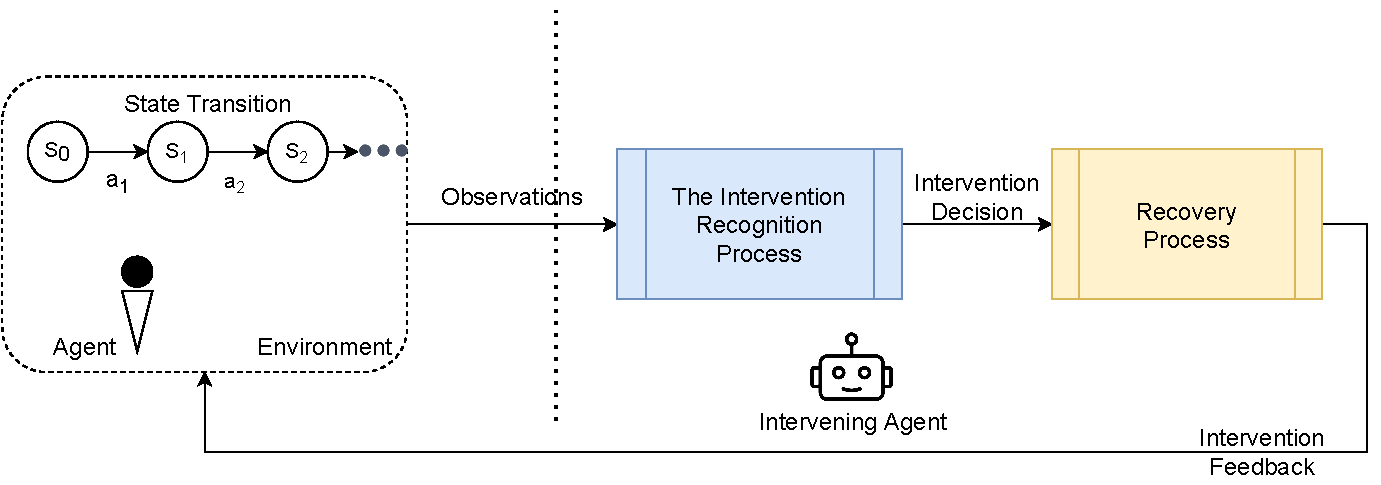
\includegraphics[width=\columnwidth]{img/interventionrecognition.pdf}}
   \caption{The stages of intervention}
\label{fig:stages}
\end{figure}

The second stage of the intervention process is \textit{\textbf{the intervention recovery process}}. 
It is natural to envision the intervention decision to manifest as an alert message for the agent in the intervention feedback loop. 
The simplest case of helping the user through intervention is to adopt a preventive measure such as blocking the recognized dangerous action or displaying an alert.
This approach makes sense in domains like cyber-security because once the attack is complete, reverting back to a safe state may be difficult. 
Furthermore, the user may not even be aware that an attack has taken place until long after. 
Examples of intervention actions include: cleaning attachments of a particular type, updating a software version or installing a firewall. 
In other domains, the preventive measures may not be as helpful. 
For example, if the intervention occurs when the human user is learning to use a new software application, the observer in addition to blocking the action, must also help the user in framing the decision about what to do next.
Therefore, in the intervention recovery process, we ask the question: \textit{can we improve the intervention recovery process to guide the user toward a desirable outcome while avoiding undesirable outcomes instead of blocking actions?} 
This is an important question, specially in cases where the agent is a human user. 
To answer this question, we present an \textbf{intervention feedback technique built on automated planning} to safely guide the user toward the goal.
The intervention feedback technique helps a human user complete a cognitively engaging problem solving task by providing helpful hints. 
A hint is a piece of information about the search problem the user is solving. 
We design helpful hints to allow the user to carefully probe the solution space of the problem during the search, while avoiding the undesirable consequence.
In this dissertation, we explore how automated planning can be used in:
\begin{itemize}
\item modeling the intervention environments
\item undesirable state recognition process
\item intervention recovery process
\end{itemize}
Automated planning is integral to the design of the intervening agent. 
First, planning is used to model the intervention environment as a state transition system comprised of preconditions and post-conditions of actions. 
Second, to achieve some goal in the environment, the user executes many actions; while a few of them incur risk, some are pivotal in triggering the undesirable consequence. 
Therefore, in order to identify when intervention is needed the observer must be able to generate alternative plans to find the many possible ways to reach the undesirable consequence. 
Third, when intervention occurs the user may still be incapable of deciding what to do next on his own, mainly because of hidden information about the domain or the actions of an adversary that the user can not control. 
Therefore, planning can be used to implement preventive measures such as blocking. 
Once the paths leading to an undesirable consequence have been identified, the planner can be provided with intervention actions that negates the states leading to the undesirable consequence. 
The preconditions of an intervention action are  states that are on the path to the undesirable consequence and the post-conditions of the intervention action negates that specific state. 
In situations where the user needs more help than a simple preventive measure, as we will show in this dissertation, automated planning can be used to help guide the user toward a plan that avoids the undesirable consequence.
Good intervention actions are those that block multiple undesirable consequences, are low cost to execute and do not interfere with the user’s needs or preferences. 
In this dissertation, we discuss three intervention models that address two of the aforementioned requirements, blocking multiple undesirable consequences and not interfering with the user's needs. 
\begin{description}
\item [Recognition of actions that ensures safety while allowing some freedom for the user : ] The observer and the user operate in an unfamiliar and online environment, where partial knowledge about the environment precludes the user from recognizing an unsafe state. 
The observer has knowledge about the user's desirable goal and the unsafe state the user likes to avoid.
We discuss the design of an observer that can intervene and guide a user toward a desirable outcome while avoiding undesirable outcomes or frustration.
When recognizing where intervention is required, the observer considers both the user's goal and the undesirable state.
Furthermore, the observer needs to allow the user reach his goal and not be constantly interrupted.
We present two intervention models that combine automated planning and machine learning. 
The observer can adopt these models to help the user reach the desirable goal while avoiding the undesirable state.
\item [Recognition of actions that enable multiple undesirable consequences : ] Using a cyber-security application, we study intervention when the observer is not aware of the user's goal, but still needs to help the user avoid multiple undesirable states in the environment. 
Because the user's goal is unknown, the observer cannot determine when to intervene based on the user's goal and the undesirable state. Therefore, we frame the observer's decision to recognize when intervention is required as a function of objective metrics. The objective metrics capture the timeliness and criticality of actions that must be flagged for intervention in order to help the observer identify at an opportune time, the actions that may cause the most damage. 
We also investigate how the missing and extraneous actions in the observation trace affects the intervention decision.
\end{description}
In both recognition types, the observer must deal with a trade-off in early recognition of potential danger versus certainty that the undesirable effects will occur. 
In this dissertation, we investigate different metrics to capture that trade-off and how to combine different objective metrics to identify pivotal actions.

\section{The Dimensions of an Intervention Problem}
Let us now look at an example application that requires intervention.
Figure \ref{fig:episode} models an application in the Blocks World domain \cite{gupta1992bw}, where two agents: a user and a competitor stack blocks to spell the words BAND and BRAND respectively.
In the environment, the user and the competitor perform the actions \textsc{pick-up}, \textsc{unstack}, \textsc{stack}, and \textsc{put-down} using the blocks A, B, N, D and R. 
The user can not recognize the block R.
The competitor uses the hidden block R to subvert the user's goal BAND and achieve his goal BRAND.
We refer to the user's goal BAND as the desirable goal (\desired) and the competitor's goal BRAND as the undesirable state (\undesired).
When the competitor and the user present actions to the observer, the observer must help the user achieve BAND while avoiding BRAND. 
The observer does this by accepting actions that help the user advance toward the goal BAND and rejecting the actions that do not. 
In this example, when the user first presents the action \textsc{unstack a b}, the observer asks the question: ``\textit{will the user avoid the undesirable state if the presented action \textsc{unstack a b} is accepted as an observation}?''
If the observer's analysis finds that the user will not avoid the undesirable state, then intervention occurs and the process moves on to the intervention recovery phase.
In the intervention recovery phase, the observer accepts actions that help the user advance toward \desired and rejects actions that enables or satisfies the undesirable state.
The actors continue to present actions until the user achieves \desired.
The observer makes the intervention decisions in favor of the user for each presented action.
\begin{figure}[ptb]
  \centering
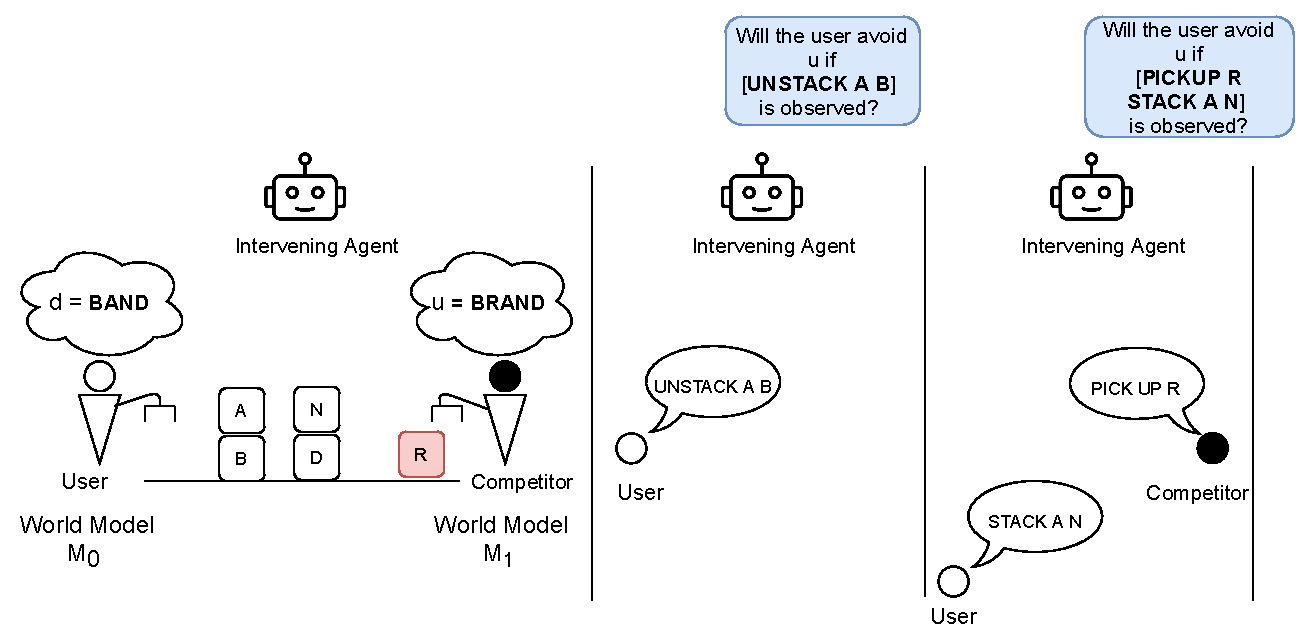
\includegraphics[width=\columnwidth]{img/episode.pdf}
\caption{An intervention episode modeled in the Blocks Words domain}
\label{fig:episode}
\end{figure}

We study several properties in the intervention environment in order to discuss the dimensions of an Intervention Problem, taking a cyber-security application and a cognitively engaging puzzle solving task as examples.
\begin{description}
\item [Actors in the environment :] The observer may be monitoring the user working alone or the user working with other agents in the domain. 
The example in Figure~\ref{fig:episode} shows a scenario where the observer monitors two actors. 
The intervention models we discuss in this dissertation consider both single agent and multi-agent intervention.
When there are other agents working to achieve goals that are different to the user's, the observer must  analyze how the post conditions of the other agents' actions affect the user's goal achievement. 
We can not assume that only the other agent's actions will always result in the undesirable state.
Sometimes, the other agents may execute actions that enable the undesirable state, but the undesirable state does not actually manifest until much later, possibly when the user executes an action that appear to be harmless. 
For example, consider a phishing attack. 
The attacker enables the attack vector by sending the phishing email to steal the user's password. However, the user's password does not get stolen until the user clicks on the link (normally, a  harmless action) to visit the phishing site and submits the information.
Recognizing these enabling actions allows the observer to intervene the user in advance and give the user some time to recover.
\item [Goals hidden to the observer :] To help the user trade-off benefits versus risks, the observer needs to know what the user thinks he/she is trying to accomplish.  
Using automated planning, we can categorize goals of the user and other actors in the environment in terms of  actions and their post conditions. 
However, in certain cases, specifying the user's goal may be difficult. 
For example, consider a home computer user preparing a document to send as an attachment in an email, while listening to music. 
In this situation, the home computer user will not be able to explicitly state his goals as post conditions of actions to the observer as required by planning.
At different times, the human user may change the order in which he wants to achieve the goals. 
For example, at the start he may want to play music in the background (as a secondary goal) while preparing the document (primary goal).
However, if he hears a song he doesn't like he may want to pause the document preparation task and change the song on the music player.
In this situation, the user's priorities change.
Therefore, in certain cases, the observer must also be able to make the intervention decision considering only the undesirable states the user wants to avoid.
\item [Types of observations :] In the example shown in Figure~\ref{fig:stages}, the observer makes the intervention decision based on actions presented by the actors. 
We make the differentiation between observations of actions and observations of state because in some intervention scenarios, the observer may not be able to observe the action itself but will be able to perceive the post conditions of the action in the environment. 
For example, consider the situation where a remote attacker sends a phishing email to the user. The observer may not be able to observe the action of sending the email.
However, the post condition of that remote action, i.e., the presence of the phishing email in the user's inbox, can be perceived by the observer.
When the actions are unobservable, the states resulting from actions can be used to extract the information necessary for the intervention decision.
Our intervention models consider both the observations of actions and states to decide when to intervene.
\item [Noise in observations :] When an agent or a human user executes actions to achieve a goal, lots of extraneous actions can be thrown into the observation trace. 
This is because the user does not intentionally want to trigger the undesirable state. Rather, he is trying accomplish a different (and useful) goal in the domain. 
This means that the plans that lead to the undesirable states may not encompass the user's goal and as a result, the observations will contain not only the undesirable actions, but also the desirable actions.
In addition to extraneous actions, the observer may miss some actions executed by the actors because of faulty sensors. 
Using the cyber-security domain as case study, we explore the impact of noise in the observation trace in making a correct intervention decision.
\item [Intervention recovery :] In this work, we model the observer as an agent who can intervene to help the user reach the desirable goal safely. We present two intervention models with different intervention recovery processes.
In one form of intervention, the observer considers the remaining plans in safe and unsafe partitions to learn to recognize unsafe suffixes in order to help the user avoid the undesirable state.
In this case, the observer can help the user by only accepting actions into the observation history that will safely advance the user toward the user's desirable goal.
In the second form of intervention, the observer learns to recognize that the user is not making progress toward \desired by analyzing the observation history when a suffix is not available. In this case,  the observer must offer enough help to \textit{guide} the user toward \desired without giving the solution. 
The second intervention model is particularly useful when the user is a human and it can be difficult evaluate progress with heuristics like a normal planning agent.
\end{description}


\section{Intervention Use Cases}
Users perform many actions in order to complete a task; while a few of them incur much risk, some are pivotal in triggering vulnerabilities. 
Given there are necessary preconditions in the system, either created by the user or by an adversary, any seemingly harmless action can suddenly become dangerous. 
The Intervention models allow us to automatically detect such vulnerable situations.
We discuss helpful intervention using two use cases. 
The uses cases we selected to study intervention have different dimensions. 
Table \ref{tab:properties} summarizes the intervention dimensions for each domain.
\begin{table}[tpb]
\caption{Dimensions of intervention use cases}
\label{tab:properties}
\resizebox{\columnwidth}{!}{%
  \begin{tabular}{|l|l|l|}
\hline
& \multicolumn{2}{c|}{\textbf{Domain}}  \\ \cline{2-3} 
\multicolumn{1}{|c|}{\textbf{Dimension}} &
  \multicolumn{1}{c|}{Cyber-security} &
  \multicolumn{1}{c|}{Rush Hour} \\ \hline
Actors in the environment  & User, Attacker, Observer & User, Observer \\ \hline
Goals hidden to the observer &
  \begin{tabular}[c]{@{}l@{}}User's goal is hidden\\ 
  Multiple known undesirable states \end{tabular} &
   \begin{tabular}[c]{@{}l@{}}User's goal is not hidden\\ 
  One or more known undesirable states \end{tabular} \\ \hline
Types of observations &
  \begin{tabular}[c]{@{}l@{}}The observer observes user's actions\\ 
  The observer only observes the effects of the attacker's actions\end{tabular} &
  The observer observes user's actions \\ \hline
Noise in observations     & Has missing and extraneous observations & None                           \\ \hline
Intervention recovery  & block action & Offer helpful hint   \\ \hline
\end{tabular}%
}
\end{table}

\subsection{Intervention in Cyber-security}
In the cyber-security domain, we model an attacker attempting to trick the user into compromising his security/privacy during day-to-day computing tasks.
The attacker creates opportunities for phishing and malware attacks by making them to appear as common harmless tasks such as email and installing software.
Unable to recognize these attacks in advance, the user becomes an unwitting accomplice to security breaches. 
The Intervention Problem for the cyber-security domain consists of three actors: the human user, the attacker (human/machine) and the observer. 
In most cyber-security cases, the attacker does not operate as a typical adversary (e.g., taking turns with the user). 
Instead the attacker takes preemptive actions and lays traps (e.g., send phishing email), which are often tied to typical actions the user performs (e.g., checking email). 
We model the cyber-security domain with multiple undesirable states: phishing attacks, malware installations. However, the user's goal is hidden to the observer.
In the cyber-security domain we model noisy observations in terms of missing and extraneous actions.
The observer considers the actions of the user and the post-conditions of attacker's actions to produce the intervention decision. 
The observation trace will contain varying noise levels from missing and extraneous actions.
Our helpful intervention solution for cyber-security is based on automated planning and uses the properties of a planning problem to identify ``\textit{critical trigger actions}'', that will cause the security breach. 
We do not study a specific recovery process for Cyber-security domain. 
We assume that when the observer identifies the critical trigger action, it is blocked.

\subsection{Intervention in Rush Hour}
Our second case study is a puzzle solving task called Rush Hour, which simulates a parking lot. In the standard version of the puzzle, the player has to clear a path on a board to move a target vehicle to the exit. To simulate the condition where the user is working only with partial knowledge about the domain, we introduced a hidden forbidden vehicle to the Rush Hour puzzle, which if moved will cause the undesirable state. 
We use the Rush Hour puzzle to approximate the case where human users learn to use a new software application and also it helps motivate the users to actually do the task in experiment conditions. 
The Rush Hour domain only has the human user and the observer. 
Unlike the cyber-security use case, the observer is aware of the desirable goal the user is trying to achieve (i.e., solve the puzzle by moving the target vehicle to the exit) and also the undesirable state (i.e., forbidden vehicle moves).
Similar to the cyber-security use case, the Rush Hour domain also contains multiple undesirable states. All states resulting from legal moves of the forbidden vehicle are undesirable.
The observations are actions the user executes to solve the puzzle. In this case, the observations are not noisy.
Our intervention solution for this case uses machine learning algorithms to recognize when the user is about to move the forbidden vehicle and intervene.
As the recovery process, we explore how to help the human user decide what to do next by offering further assistance as helpful hints.
In both cases the user actively pursues his own goal. 
The threats are triggered because the user did not understand the consequences of reaching the undesirable state (phishing/malware vulnerabilities) or was not aware of the undesirable state from the start (hidden forbidden vehicle in Rush Hour). 
The observer makes the decision to intervene upon recognizing actions in the observations that enable or satisfy the undesirable state.
 
\section{Distinguishing Intervention From Plan Recognition}
Plan recognition is the closest to our Intervention Problem. 
In the literature the plan recognition is defined as the problem of taking as input a sequence of actions performed by an actor and inferring the goal pursued by the actor and also organizing the sequence as a plan structure \cite{kautz1986generalized,schmidt1978}. 
The solution to the plan recognition problem is given by the set of goals that produces a plan that is compatible with the observations. 
The online version of the plan recognition problem uses observations as they happen as input. 
The offline version requires the complete observation to be available in advance. 
At first glance, it might seem that intervention is a variant of Plan Recognition for the user's desirable goal and the undesirable states the user wants to avoid. 
However, there are several subtleties that make intervention unique, which we now discuss.
\begin{itemize}
\item \textbf{Intervention is an online problem.}
In most cases Plan Recognition (e.g., \cite{ramirez2009plan,ramirez2010probabilistic, sohrabi2016plan}) is an offline problem;
there are a few notable exceptions \cite{mirsky2018}.
However, intervention is inherently online and dynamic.  
The observer decides whether to intervene (or not) every time the user(s) presents an action.
In order to make the decision, the observer uses the observation history, which contains accepted actions.
Intervention is a multi-agent problem as well. 
This has ramifications in environments where the user and the competitor compete to achieve close but different goals. 
With intervention, the observer can help the user by accepting actions into the observation history that only help further the user's goal. 
This is not possible with offline plan recognition.
\item \textbf{Agents may have distinct views of the problem.}  
The user and the competitor are modeled with different domain definitions. 
When the agents have distinct views of the problem and they can not satisfy the undesirable state on their own, conditions will arise such that the agents working together will enable the undesirable state.
The user wants to satisfy the desirable goal state, while avoiding the \textit{hidden} undesirable state.
The competitor is trying to subvert the user’s goal by enabling preconditions for the undesirable state without the user's knowledge.
When the user and the competitor reveal their plan(s) incrementally, the observer needs to decide whether the revealed actions make it impossible for the user to avoid the undesirable state considering the plans from the user's and the competitor's domain definitions collectively. 
Any action that make it impossible for the user to avoid the undesirable state must be flagged for intervention and not accepted into the observation history.
If the plans for the undesirable state and desirable goal share a long common prefix, 
it will be difficult for the observer to disambiguate between the goals and to use plan recognition algorithms in time to help the user avoid the undesirable state.
\item \textbf{Partitioned suffixes (with known desirable goal).}
When the desirable goal is known, the observer should allow the user to pursue suffixes leading to the desirable goal and intervene when actions are presented from suffixes that get ``too close'' to the undesirable state. 
Our key insight is to model the  ``goals'' of the user and competitor, which justifies our use of planning to find these suffixes. 
However, intervention adds new concerns beyond plan recognition, namely that the observer needs to consider two kinds of goals that might require intervention:
\begin{enumerate}
\item Cases where the user is headed toward a undesirable outcome. 
This can be easily be solved by plan recognition.
\item Cases where the user unwittingly enables an undesirable outcome by taking actions toward a desired goal. 
This is less easily solved by plan recognition because there is an inherent trade-off between intervening and allowing the user some freedom to pursue the desirable goal. 
Suppose that some suffix $\Suffix_{\undesired}$ leads to the undesirable state and suffix $\Suffix_{\desired}$ leads to the desirable goal.  
Then it can happen that by simply following the plan leading to the desirable goal, the user enables the undesirable state when there is enough overlap between  $\Suffix_{\undesired}$ and $\Suffix_{\desired}$.
\end{enumerate}
Partitioning the suffixes this way allows the observer to learn the differences between the safe and the unsafe suffixes and balance specific unsafe actions with those that are necessary for allowing the user some freedom.
For example, in a malicious email attack such as phishing, the user will still want to check email.
So prohibiting email is untenable; what the agent must do is intervene when the user attempts to click the phishing link.
This need for partitioning the suffixes  is distinct from plan recognition, where existing offline Plan Recognition algorithms often rely on  plan cost to disambiguate between goals and recognize suffixes. 
When the undesirable state and the desirable goal are too close, disambiguation based on plan cost will not work (we will demonstrate in a later chapter). 
Learning the differences between the plan partitions will allow us to address this issue.
\item \textbf{Suffix analysis with unknown desirable goal.}
When the desirable goal is unknown, the observer only has the space of plans leading to the undesirable goals to make the intervention decision when the agents reveal their plans incrementally.
Plan recognition over the undesirable goals does not really     apply because it is     focused on matching actions to  prior plans     to determine the goals the      user is trying  to achieve.     
In other words, the observer assumes that the user is executing some plan to reach the undesirable state.
In reality, the user wants to avoid the undesirable state and reach a different (desirable) goal, which may be unknown to the observer.
Therefore, when analyzing partition suffixes with known desirable goal, the observer uses the knowledge of the user's goal to determine which are critical actions that require intervention.   
In contrast, with unknown desirable goal, the observer analyzes the remaining undesirable suffixes to identify actions that cause the most damage to intervene the user.
\item \textbf{Goal priors cannot be estimated reliably.}  
Plan Recognition algorithms use a prior probability distribution over the goal hypotheses to estimate the posterior probability of the likely goals given the observations. 
Intervention must consider the likely goals regardless of their priors. 
For example, the undesirable state is hidden from the user, who does not intend to achieve it (i.e., prior probability $\approx 0$). 
In contrast, a competitor, when present, intends to achieve the undesirable state (i.e., prior probability $\approx 1$).
When the priors are not accurate, the observer (using Plan Recognition) may not be able to  disambiguate between likely goals (and recognize the correct plan) in time to avoid the undesirable state.
  
\item \textbf{Emphasis on intervention recovery.}
In Plan Recognition, the observer uses an observation trace to derive the user's likely plan. 
The observation trace can be either an ordered sequence of actions  \cite{ramirez2009plan,ramirez2010probabilistic} or an ordered sequence of states \cite{sohrabi2016plan}.
Plan Recognition does not define a method for the user to recover when the observer recognizes a plan leading to the undesirable state. 
With the proposed intervention models, we address that limitation with two different types of help the observer can offer to the user to decide what to do next.
\end{itemize}


\section{Research Questions}
The main objective of this research is to study different intervention models that help human users complete tasks safely. We address the following research questions: 
\begin{description}
\item[What are the salient characteristics for deciding when to intervene?]
We address this question considering the dimensions of an intervention problem, summarized in Table~\ref{tab:properties}.

Our intervention models are based on identifying actions in an observation trace that either satisfy the undesirable state or enable it. 
This requires the observer to evaluate the current state (i.e., state resulting from the observed actions) based on it's importance to causing the undesirable state considering the user's desirable goal (if available) and the undesirable state.
In the two intervention use cases, criticality of the current state is evaluated using two different methods. 
For the cyber-security domain we identify salient features by analyzing the plan space. 
We model the cyber-security domain as a planning problem and use an existing automated planner to  sample the possible solutions (plans) that project possible undesirable outcomes and then trace back to actions critical to their occurrence. 
The resulting plans are analyzed to extract objective metrics to predict if the current action is likely to trigger the undesirable consequences. 
Raising a warning to the user involves a trade-off in early recognition of potential danger versus certainty that the effects will occur. 
We investigate different objective metrics to capture that trade-off and how to combine these objective metrics to identify pivotal actions. 

To study intervention in the Rush Hour domain, we formalize a family of Intervention Problems and show how these problems can be solved using a combination of Plan Recognition methods and classification techniques to decide whether to intervene. 
We characterize the observer's decision space as an Intervention Graph and construct it using an ``Intervention as Classical Planning'' approach to generate potential suffixes of partially executed plans. 
We extract domain-independent features from this graph and extend several Plan Recognition benchmarks to evaluate this approach. 
We then generalize these results to Human-Aware Intervention, where the observer must decide in
real time whether to intervene for human users solving a cognitively engaging puzzle. 
Using a revised feature set more appropriate to human behavior, we produce a learned model to recognize when a human user is about to trigger an undesirable outcome.

\item[How should information be displayed to effectively inform users following intervention?] Using the Rush Hour domain, we study how an intervention model can be extended to help users continue a cognitively engaging task by providing helpful hints. 
In the context of the Rush Hour puzzle solving task, a hint is a piece of information about the Rush Hour search problem. 
We design helpful hints to allow the user to carefully probe the search space of the Rush Hour search problem, while avoiding the undesirable state.
We monitor how human users achieve planning landmarks of the Rush Hour problem when intervention is supported by hints compared to intervention without hints to evaluate the effectiveness of our intervention recovery process.

\item[How to design tools to study intervention in activities with human user participation?]
To identify pivotal events, the appropriate system states and user actions must be monitored and compared to a model of actions that can lead to the undesirable state. 
If an action that contributes to a trigger is suspected, it should be put in the context of what the user is trying to do and an estimate of how likely the action is to actually cause the undesirable state. 
We develop state/action models using automated planning that allow us to recognize the appropriate system \textit{states} (computer/puzzle board) that must be monitored and the \textit{actions}, which may lead to the undesirable state. 
For the cyber-security domain, we model the security vulnerabilities that occur in a home computer environment using PDDL (Planning Domain Definition Language) \cite{ghallab1998}, which is designed to represent pre-conditions and post-conditions of actions. 
PDDL is the prominent representation used in the AI Planning community. 
We also develop PDDL models for the Rush Hour domain, which will be used in generating the helpful hints. 
Our studies are focused on how human users solve these tasks (e.g., perform common home computer user actions, solve a Rush Hour puzzle), which requires studying human users in situ. 
To this end, we will develop a simulated home computer environment for studying users practice computer security and a Rush Hour puzzle simulator to study how human users respond to helpful hints. 
Both these tools are event monitoring systems that capture human user's actions when placed in different experimental conditions as well as system level events that are defined in the PDDL models.
\end{description}


The rest of this dissertation is organized as follows:
\begin{itemize}
\item \textbf{Chapter 2}: We present the background on automated planning and a review of existing plan recognition literature that studied methods to infer an agent's intention.
\item \textbf{Chapter 3}: We present the findings of an human subject study to motivate plan intervention. In this study, we simulate cyber-security vulnerabilities that occur in a home computer environment when the human users perform routine tasks like checking email and using software applications.
\item \textbf{Chapter 4}: We present the first intervention model based on the findings of the cyber-security human subject study. 
We formulate the Intervention Problem as a  planning problem of three domain independent objective metrics: timeliness, which captures how soon the undesirable state may occur; certainty, which captures how frequently the undesirable state may be seen; and desirability, which captures the user’s preference for continuing the current action despite the increased risk. 
Against an ideal baseline, we examine trade-offs in choosing the ``correct'' intervention point by varying the weights associated with these objective metrics, the observability of actions, and the presence of extraneous actions.
\item \textbf{Chapter 5}: We study two kinds of Intervention Problems in environments where an observer monitors a user (and a competitor) and help the user achieve a desirable goal, while avoiding an undesirable state. 
In ``\textbf{Unsafe Suffix Intervention}'', the observer uses automated planners to project the remaining suffixes and extract features that can differentiate between safe and unsafe plans. 
We evaluate the recognition accuracy of Unsafe Suffix Intervention on benchmark planning
problems. 
In ``\textbf{Human-aware Intervention}'', the observer uses the observed partial solution to extract features that can separate safe and unsafe solutions. 
We evaluate the accuracy of Human-aware Intervention on a new Intervention Planning benchmark Rush Hour.
\item \textbf{Chapter 6}: We present an intervention recovery process for the Human-aware Intervention model based on automated planning. 
We discuss the findings of a human subject study where human users solved a cognitively engaging Rush Hour puzzle task while being guided by a human-aware intervention agent. 
We evaluate the efficacy of our recovery approach using automated planning landmarks.
\item \textbf{Chapter 7}: We discuss some open issues in Intervention and provide an outline for future research.
\end{itemize}
